%%%%%%%%%%%%%%%%%%%%%%%%%%%%%%%%%%%%%%%%%
% Beamer Presentation
% LaTeX Template
% Version 1.0 (10/11/12)
%
% This template has been downloaded from:
% http://www.LaTeXTemplates.com
%
% License:
% CC BY-NC-SA 3.0 (http://creativecommons.org/licenses/by-nc-sa/3.0/)
%
%%%%%%%%%%%%%%%%%%%%%%%%%%%%%%%%%%%%%%%%%

%----------------------------------------------------------------------------------------
%	PACKAGES AND THEMES
%----------------------------------------------------------------------------------------

\documentclass{beamer}

\mode<presentation> {

% The Beamer class comes with a number of default slide themes
% which change the colors and layouts of slides. Below this is a list
% of all the themes, uncomment each in turn to see what they look like.

\usetheme{default}
%\usetheme{AnnArbor}
%\usetheme{Antibes}
%\usetheme{Bergen}
%\usetheme{Berkeley}
%\usetheme{Berlin}
%\usetheme{Boadilla}
%\usetheme{CambridgeUS}
%\usetheme{Copenhagen}
%\usetheme{Darmstadt}
%\usetheme{Dresden}
%\usetheme{Frankfurt}
%\usetheme{Goettingen}
%\usetheme{Hannover}
%\usetheme{Ilmenau}
%\usetheme{JuanLesPins}
%\usetheme{Luebeck}
%\usetheme{Madrid}
%\usetheme{Malmoe}
%\usetheme{Marburg}
%\usetheme{Montpellier}
%\usetheme{PaloAlto}
%\usetheme{Pittsburgh}
%\usetheme{Rochester}
%\usetheme{Singapore}
%\usetheme{Szeged}
%\usetheme{Warsaw}

% As well as themes, the Beamer class has a number of color themes
% for any slide theme. Uncomment each of these in turn to see how it
% changes the colors of your current slide theme.

%\usecolortheme{albatross}
%\usecolortheme{beaver}
%\usecolortheme{beetle}
%\usecolortheme{crane}
%\usecolortheme{dolphin}
%\usecolortheme{dove}
%\usecolortheme{fly}
%\usecolortheme{lily}
%\usecolortheme{orchid}
%\usecolortheme{rose}
%\usecolortheme{seagull}
%\usecolortheme{seahorse}
%\usecolortheme{whale}
%\usecolortheme{wolverine}

%\setbeamertemplate{footline} % To remove the footer line in all slides uncomment this line
%\setbeamertemplate{footline}[page number] % To replace the footer line in all slides with a simple slide count uncomment this line

%\setbeamertemplate{navigation symbols}{} % To remove the navigation symbols from the bottom of all slides uncomment this line
}

\usepackage{graphicx} % Allows including images
\usepackage{booktabs} % Allows the use of \toprule, \midrule and \bottomrule in tables
\usepackage{subcaption}
\usepackage{caption}

%----------------------------------------------------------------------------------------
%	TITLE PAGE
%----------------------------------------------------------------------------------------

\title[]{{\tiny{ME 766 Course Project}}\\Parallelization of Advection Scheme using MPI} % The short title appears at the bottom of every slide, the full title is only on the title page

\author{Saran S - 133106001 \\ Rahul Joshi - 133106002} % Your name
\institute[Indian Institute of Technology, Bombay] % Your institution as it will appear on the bottom of every slide, may be shorthand to save space
{
Indian Institute of Technology, Bombay \\ % Your institution for the title page
\medskip
\textit{} % Your email address
}
\date{\today} % Date, can be changed to a custom date

\begin{document}

\begin{frame}
\titlepage % Print the title page as the first slide
\end{frame}

\begin{frame}
\frametitle{Problem Description} % Table of contents slide, comment this block out to remove it
\begin{figure}
\centering
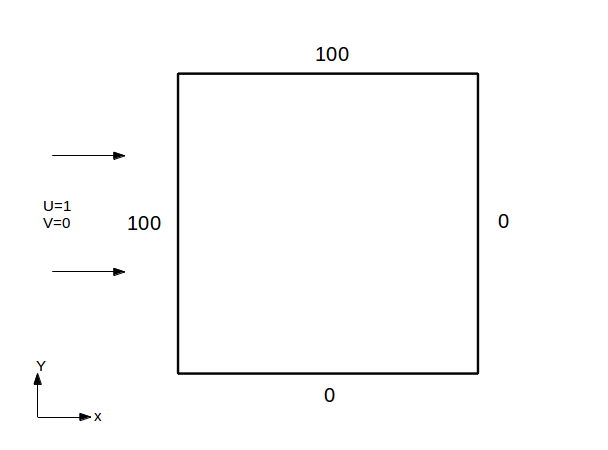
\includegraphics[width=0.7\textwidth]{1} % Throughout your presentation, if you choose to use \section{} and \subsection{} commands, these will automatically be printed on this slide as an overview of your presentation
\caption{Schematic of advection problem}
\end{figure}
\end{frame}

%----------------------------------------------------------------------------------------
%	PRESENTATION SLIDES
%----------------------------------------------------------------------------------------

%------------------------------------------------
%\section{First Section} % Sections can be created in order to organize your presentation into discrete blocks, all sections and subsections are automatically printed in the table of contents as an overview of the talk
%------------------------------------------------

%\subsection{Subsection Example} % A subsection can be created just before a set of slides with a common theme to further break down your presentation into chunks

\begin{frame}
\frametitle{Implementation methods}
\begin{itemize}
\item Serial vectorised Python code using Numpy module
\item Using Python MPI library mpi4py
\end{itemize}
\end{frame}

%------------------------------------------------

\begin{frame}
\frametitle{Vectorised code}
\begin{itemize}
\item Non-vectorised code : Single pair of operands at a time
\item Vectorised code : Multiple pair of operands at a time
\end{itemize}
\end{frame}

%------------------------------------------------
\begin{frame}
\frametitle{Profiling}
\begin{itemize}
\item Program analysis to measure the memory and time complexity involved
\item Performed to optimize code
\end{itemize}% \\
%\vspace{0.5cm}
\pause
In our program line by line profiling has been done using Kernprof
\begin{figure}
\centering
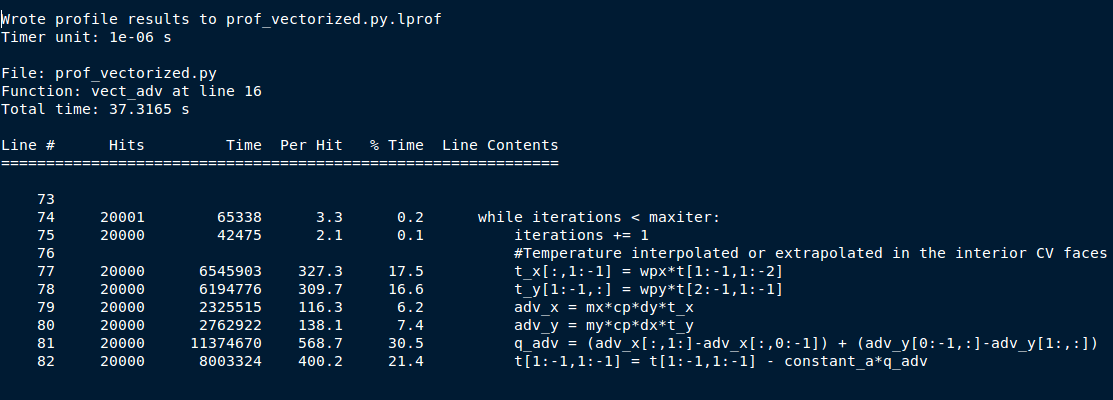
\includegraphics[width=1.0\textwidth]{profile}
\end{figure}
\end{frame}

%-----------------------------------------------
\begin{frame}
\frametitle{MPI Implementation}
\begin{itemize}
\item To utilise multiple processing elements
available based on distributed shared memory concept
\item Initiates same script on all PE's
\item PE works on a part of whole domain data
\item Data finally gathered back to root PE 
\end{itemize}
we implemented MPI library for python - \textbf{mpi4py}
\end{frame}

%-------------------------------------------------
\begin{frame}
\frametitle{Computer Specification}
\begin{itemize}
\item Hardware : Intel Core i5-2430M CPU @ 2.40GHz × 4, \\
\hspace{1.7cm} Memory 3.8 GB, L1 Cache 32K, L2 Cache 256K, \\
\hspace{1.7cm} L3 Cache 3072K
\item Software : Ubuntu 12.04, 64 bit
\end{itemize}
\end{frame}

%---------------e---------------------------------

\begin{frame}
\frametitle{Results}
\begin{figure}
\centering
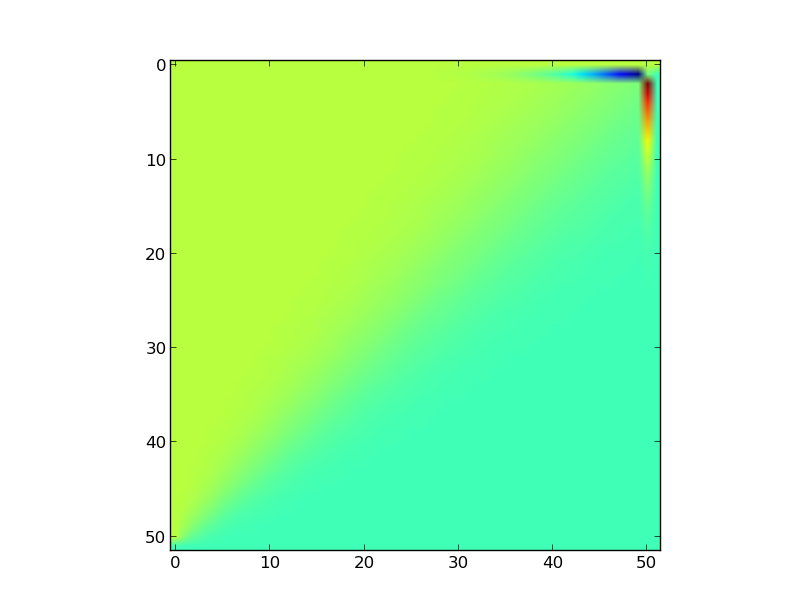
\includegraphics[width=0.7\textwidth]{image52} % Throughout your presentation, if you choose to use \section{} and \subsection{} commands, these will automatically be printed on this slide as an overview of your presentation
\caption{Solution of the advection problem}
\end{figure}
\end{frame}






\begin{frame}
\frametitle{Results}
\begin{figure}
\centering 
\begin{subfigure}{0.49\textwidth}
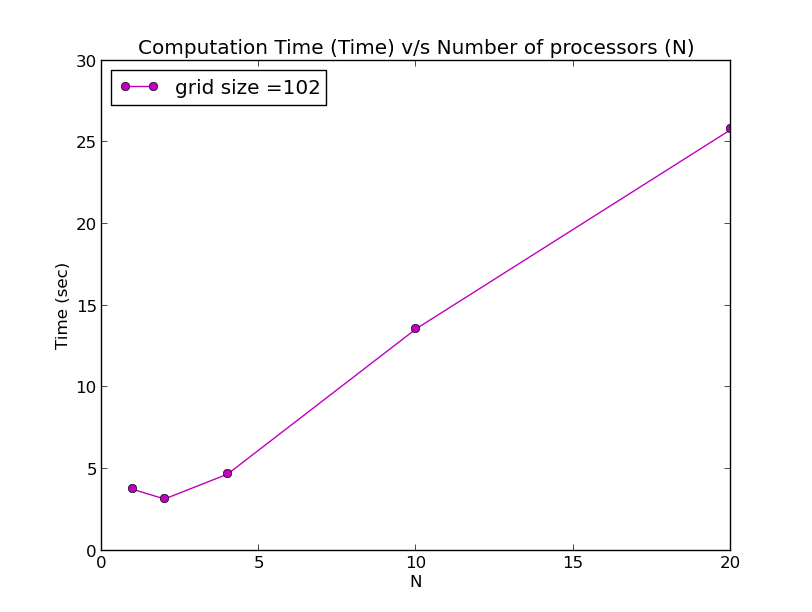
\includegraphics[width=\textwidth]{102}
\caption{Grid size 102}
\end{subfigure}
\begin{subfigure}{0.49\textwidth}
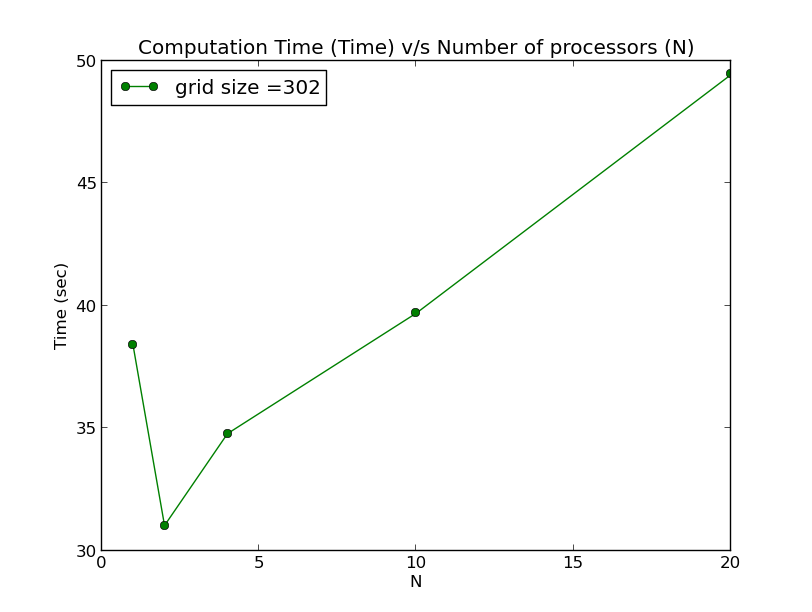
\includegraphics[width=\textwidth]{302}
\caption{Grid size 302}
\end{subfigure}
\end{figure}
\end{frame}

%------------------------------------------------
\begin{frame}
\frametitle{Results}
\begin{figure}
\centering 
\begin{subfigure}{0.49\textwidth}
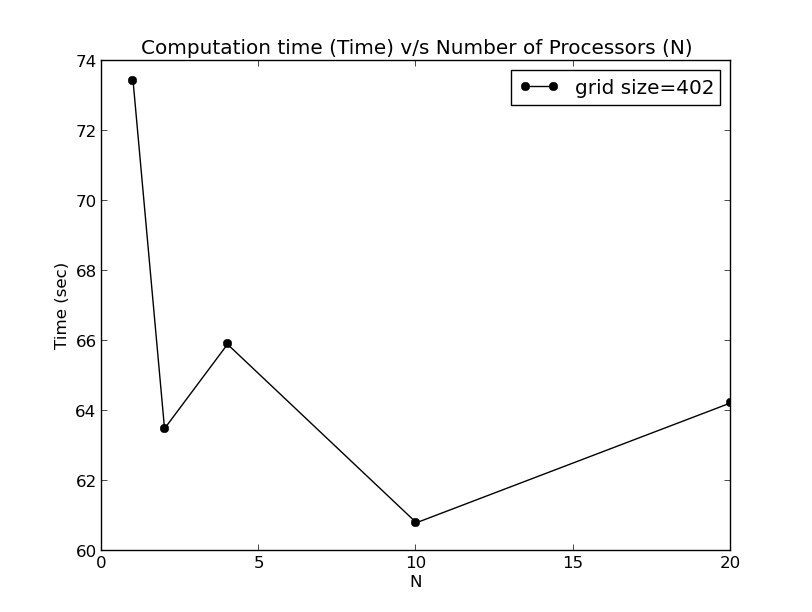
\includegraphics[width=\textwidth]{402}
\caption{Grid size 402}
\end{subfigure}
\begin{subfigure}{0.49\textwidth}
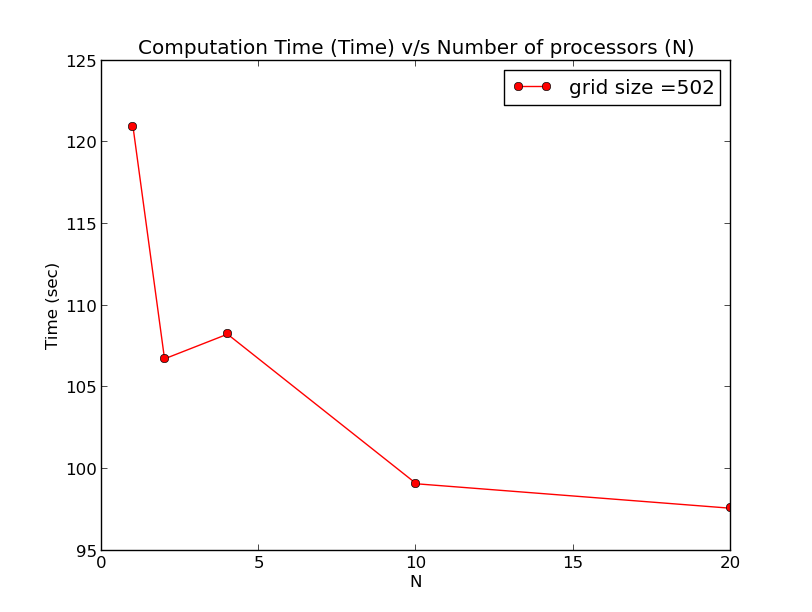
\includegraphics[width=\textwidth]{502}
\caption{Grid size 502}
\end{subfigure}
\end{figure}
\end{frame}

%----------------------------------------------------------------------------------------

\begin{frame}
\frametitle{Results}
\begin{figure}
\centering 
\begin{subfigure}{0.49\textwidth}
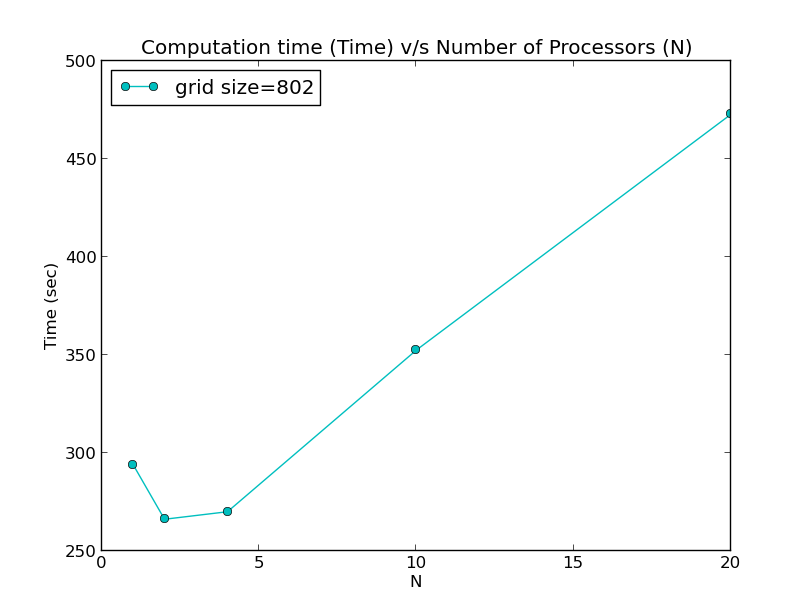
\includegraphics[width=\textwidth]{802}
\caption{Grid size 802}
\end{subfigure}
\begin{subfigure}{0.49\textwidth}
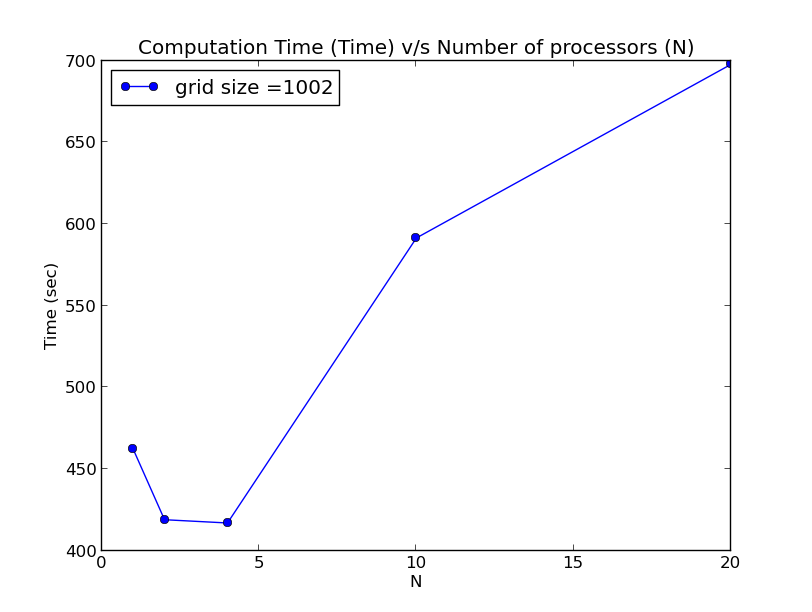
\includegraphics[width=\textwidth]{1002}
\caption{Grid size 1002}
\end{subfigure}
\end{figure}
\end{frame}


%------------------------------------------------------------------------------------

\begin{frame}
\frametitle{Conclusions}
\begin{itemize}
\item Profiling helped us to identify the portion of the code which took maximum time for computation
\item The performance for 2 and 4 PEs was as expected with increase in grid size 
\item For 10 and 20 PEs, the computation time taken was more
\item For grid size 402 and 502 there was a change in trend of the computation time
\end{itemize}
\end{frame}

\end{document} 